\documentclass[11pt]{article}

\usepackage[margin=1.7cm]{geometry}
\usepackage{amsmath}
\usepackage{amssymb}
\usepackage{enumitem}
\usepackage{titlesec}
\usepackage{xcolor}
\usepackage{fancyhdr}
\usepackage{tikz}
\usetikzlibrary{arrows.meta}
\usepackage{pgfplots}
\usepackage{multicol}
\usepackage{array}
\pgfplotsset{compat=1.18}

\titleformat{\section}{\large\bfseries}{\thesection}{0.6em}{}
\titlespacing{\section}{0pt}{1.1em}{0.5em}

\pagestyle{fancy}
\fancyhf{}
\fancyhead[L]{Year 9 Algebra Revision --- Applications}
\fancyhead[R]{Name: \makebox[4cm]{\hrulefill}}
\fancyfoot[C]{\thepage}
\renewcommand{\headrulewidth}{0.4pt}

\newcommand{\ans}{\hrulefill}
\setlist[enumerate,1]{leftmargin=1.4em, itemsep=0.6em, topsep=0.2em}
\setlist[enumerate,2]{leftmargin=1.3em, itemsep=0.4em, topsep=0.2em}
\setlength{\columnsep}{1.1cm}
\setlength{\columnseprule}{0.4pt}

\newcommand{\markpt}[3]{\filldraw (axis cs:#1,#2) circle (1.5pt); \node[#3, font=\small] at (axis cs:#1,#2) {$(#1,#2)$};}
\newcommand{\dotpt}[2]{\filldraw (axis cs:#1,#2) circle (1.5pt);}

% \gridaxis{xmin}{xmax}{ymin}{ymax}{xtick dist}{ytick dist}
\newcommand{\gridaxis}[6]{%
  \begin{axis}[
    width=7.4cm, height=6.4cm,
    xmin=#1, xmax=#2, ymin=#3, ymax=#4,
    grid=both, grid style={line width=.1pt, draw=gray!35},
    axis lines=middle,
    xlabel={$x$}, ylabel={$y$},
    xtick distance=#5, ytick distance=#6,
    tick label style={font=\tiny},
    label style={font=\small},
    xlabel style={at={(axis description cs:1,0)}, anchor=north west},
    ylabel style={at={(axis description cs:0,1)}, anchor=south east},
    axis line style={-{Latex[length=1.8mm]}},
  ]
}

\begin{document}

\begin{center}
  {\Large\bfseries Year 9 Algebra Revision --- Applications}
\end{center}
\vspace{0.3em}
\noindent\textit{Harder numbers, less scaffolding, and real-world problems. Show every step of your working.}

\vspace{0.4em}
\section{Harder Equations}
\noindent Expand brackets (watch the signs!) and collect like terms before solving.

\begin{multicols}{2}
\begin{enumerate}
  \item $3(x + 4) = 2(x + 9)$ \ans
  \item $5(x + 1) = 2(x + 7)$ \ans
  \item $20 - 3(x - 2) = 11$ \ans
  \item $15 - 2(x - 1) = x + 5$ \ans
  \item $\dfrac{x+5}{3} = 6$ \ans
  \item $\dfrac{2x-4}{3} = 4$ \ans
\end{enumerate}
\end{multicols}

\section{A Harder Pattern}
\noindent Crosses are made from square tiles. Only $n=1$ and $n=3$ are shown below --- $n=2$ is missing.

\begin{center}
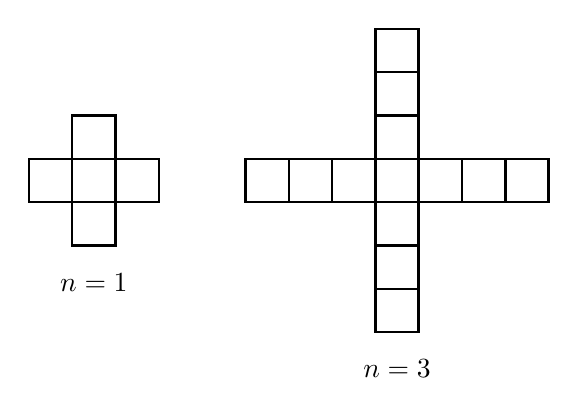
\begin{tikzpicture}[scale=0.55, line width=0.9pt]
  \draw (0,0) rectangle (1,1);
  \draw (0,1) rectangle (1,2);
  \draw (0,-1) rectangle (1,0);
  \draw (1,0) rectangle (2,1);
  \draw (-1,0) rectangle (0,1);
  \node[below] at (0.5,-1.4) {$n=1$};
  \begin{scope}[xshift=7cm]
    \draw (0,0) rectangle (1,1);
    \foreach \i in {1,2,3} {
      \draw (0,\i) rectangle (1,\i+1);
      \draw (0,-\i) rectangle (1,-\i+1);
      \draw (\i,0) rectangle (\i+1,1);
      \draw (-\i,0) rectangle (-\i+1,1);
    }
    \node[below] at (0.5,-3.4) {$n=3$};
  \end{scope}
\end{tikzpicture}
\end{center}

\vspace{0.6em}
\begin{center}
\begin{tabular}{|c|c|c|c|c|c|}
\hline
$n$ & $1$ & $2$ & $3$ & $4$ & $5$ \\\hline
tiles & $5$ & & $13$ & & \\\hline
\end{tabular}
\end{center}

\begin{enumerate}
  \item[(a)] Using only the $n=1$ and $n=3$ diagrams, how many tiles are added each time $n$ increases by 1? \ans
  \item[(b)] Complete the table above.
  \item[(c)] Write the rule: tiles $=$ \ans
\end{enumerate}

\begin{center}
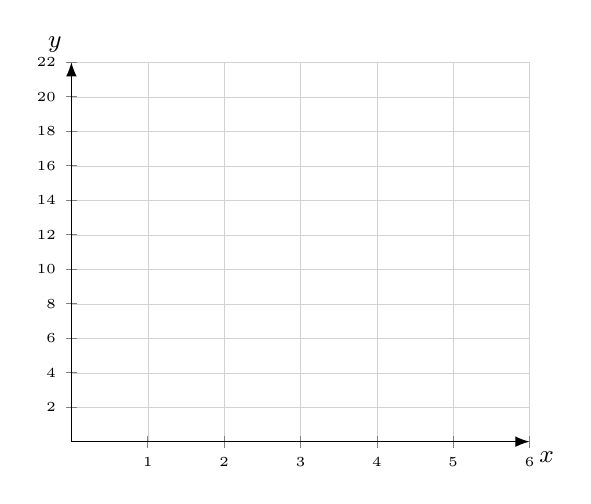
\begin{tikzpicture}
\gridaxis{0}{6}{0}{22}{1}{2}
\end{axis}
\end{tikzpicture}
\end{center}

\noindent Plot the points from your table and draw the line. Gradient: \ans \qquad $y$-intercept: \ans

\section{Application Problems}

\begin{enumerate}
  \item \textbf{Phone plan.} A mobile phone plan costs \$20 per month plus \$0.40 per minute of calls. The total monthly cost, $C$ dollars, for $m$ minutes is
  \[
    C = 0.4m + 20.
  \]
  \begin{enumerate}
    \item Find the cost for a month with 50 minutes of calls. \ans
    \item Jess's bill was \$52. How many minutes did she use? \ans
  \end{enumerate}

  \item \textbf{Filling a tank.} A water tank already contains 30 L when a hose starts filling it at a constant rate of 6 L per minute.
  \begin{enumerate}
    \item Write an equation for the volume $V$ litres in the tank after $t$ minutes. \ans
    \item Complete the table below using your equation.
    \begin{center}
    \begin{tabular}{|c|c|c|c|c|c|}
    \hline
    $t$ (min) & $0$ & $2$ & $4$ & $6$ & $8$ \\\hline
    $V$ (L) & & & & & \\\hline
    \end{tabular}
    \end{center}
    \item The tank's capacity is 90 L. Use your equation to find how long it takes to fill completely. \ans
  \end{enumerate}

  \item \textbf{Taxi fares.} A taxi company charges a fixed flag-fall fee plus a rate per kilometre. The table shows the fare for different distances.
  \begin{center}
  \begin{tabular}{|c|c|c|c|}
  \hline
  distance, $d$ (km) & $2$ & $5$ & $8$ \\\hline
  fare, $F$ (\$) & $9$ & $15$ & $21$ \\\hline
  \end{tabular}
  \end{center}
  \begin{enumerate}
    \item Find the rate per km (the gradient). \ans
    \item Find the flag-fall fee (the $y$-intercept). \ans
    \item Write the equation for the fare: $F = $ \ans
    \item Use your equation to predict the fare for a 12 km trip. \ans
  \end{enumerate}

  \item \textbf{Savings.} Maria is saving money each week. After 3 weeks she has \$85. After 7 weeks she has \$145.
  \begin{enumerate}
    \item Find how much she saves each week (the gradient). \ans
    \item Find how much she started with (the $y$-intercept). \ans
    \item Write the equation for her savings, $S$, after $w$ weeks: $S = $ \ans
    \item How much will she have after 12 weeks? \ans
  \end{enumerate}

  \item \textbf{Comparing two gyms.} Gym A charges a \$50 joining fee plus \$10 per session. Gym B charges no joining fee but \$18 per session.
  \begin{enumerate}
    \item Write an equation for the total cost at Gym A after $s$ sessions. \ans
    \item Write an equation for the total cost at Gym B after $s$ sessions. \ans
    \item Find the total cost at each gym after 6 sessions. Which gym is cheaper? \ans
    \item Find the total cost at each gym after 10 sessions. Which gym is cheaper now? \ans
  \end{enumerate}
\end{enumerate}

\end{document}
